%
\index{Logic-tree}
The logic-tree is an integral component of a PSHA input model for the 
OpenQuake-engine. 
%
An \gls{acr:oqe} input model always contains a logic tree structure 
describing the epistemic uncertainties associated with the construction 
of the seismic source model and a logic-tree used to formally specify 
epistemic uncertainties related to the \gls{acr:gsim} models used in 
different tectonic regions for the calculation of hazard.

The definition of logic trees in the OpenQuake-engine is based on
the combination of predefined modules each one modelling a specific 
epistemic uncertainty.
%
Two are the main advantages of this approach. The first and most obvious  
is that the user is not forced to use a predefined logic tree structure and
- instead - can create a tailored logic tree which integrally 
reflects the specific uncertainties he wants to model. 
%
The second is that the logic tree structure becomes an integral part of  
a PSHA input model definition. The hazard calculations based on this approach
are testable, fully reproducible and do not require pre- or 
post-processing steps since these are features included in the engine.

This Chapter is dedicated to the description of the basic theory behind 
logic-trees and to the delineation of how logic-trees are implemented 
into the OpenQuake-engine.
%
% ..............................................................................
\section{Introduction}
The use of logic-trees to account for epistemic uncertainties in  
probabilistic seismic hazard analysis was originally proposed by 
\textcite{kulkarni84}.
%
Nowadays logic-trees are an essential component of a \gls{acr:psha} input
model and represent the formal methodology though which is possible to 
synthesize the outcomes of the elicitation process on epistemic uncertainties
requested in site-specific seismic hazard analyses \parencite{budnitz1997}
as well as for the creation of state\--of\--the\--art national and 
regional \gls{acr:psha} input models. 

The interpretation of the branches in a logic tree structure, of their 
corresponding weights and of the following results is still the subject 
of an intense scientific debate going on in the literature since 2005 
\parencite{abrahamson2005,mcguire2005,scherbaum2011,musson2012}.
%
There is however a general agreement on the fact that the branches used to 
describe alternative interpretations (or values of a parameter affected by
epistemic uncertainty) must be mutually exclusive and collectively exhaustive
\parencite{bommer2008}. 
%
This means that while processing the logic tree, once you choose one option 
in the implementation of a model you automatically exclude the other possible 
interpretations (mutual exclusivity) and that the set of options described 
by the different branches represents the entire group of options admitted 
(collective exhaustiveness). 
%
While the first assumption is relatively easy to accept - although it presumes 
the lack of correlation between the uncertainties in the different branches - 
the second one certainly has implications that are more difficult and delicate 
to go along with since it presumes a comprehensive knowledge of a specific 
model uncertainty, knowledge that cannot be assumed a-priori. 
%
% -------------------------------------------------------------------->>> Figure
\begin{figure}[!ht]
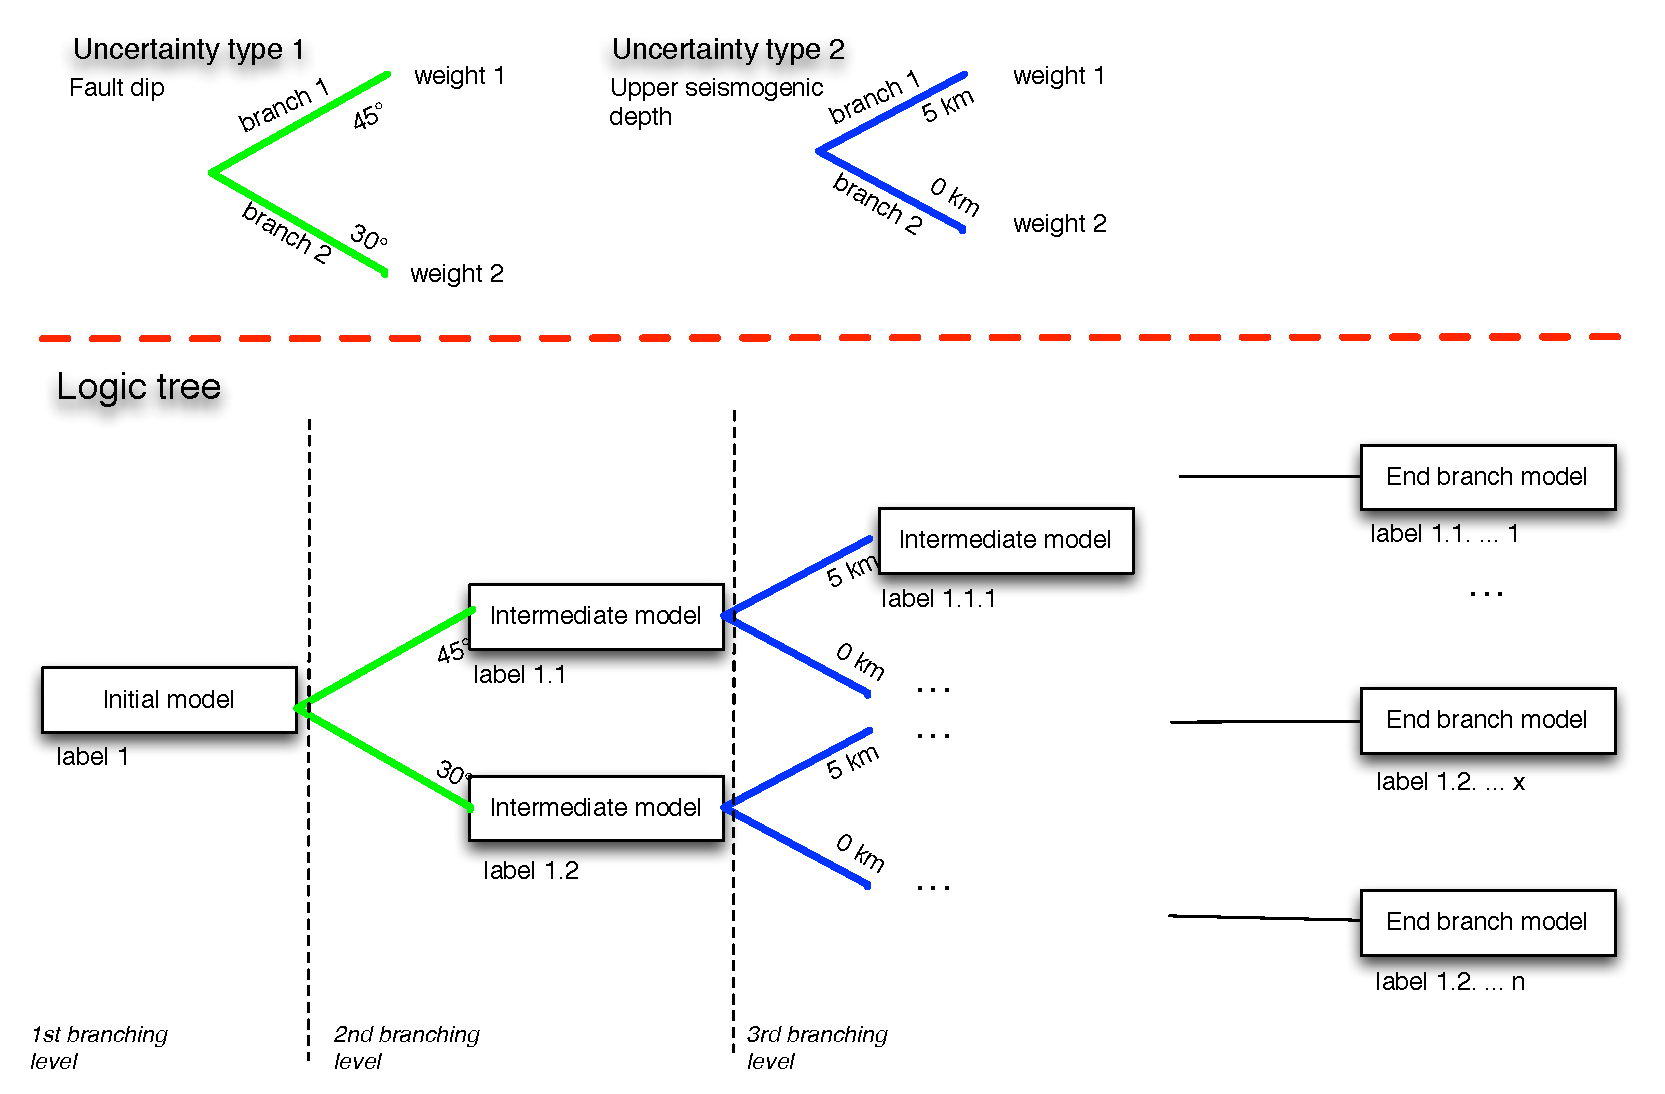
\includegraphics[width=\textwidth]{./Pictures/lts/logic_tree.pdf}
\caption{An example of modular logic tree structure supported by the
    \gls{acr:oqe}. The upper part of the figure contains two modules, one
    modelling the epistemic uncertainty on the dip angle of a fault, the 
    other modelling the uncertainty on faults upper seismogenic depth.}
\label{fig:logic_tree}
\end{figure}
% --------------------------------------------------------------------<<< Figure
%
% ..............................................................................
\section{The OpenQuake-engine logic-tree structure}
\label{sec:lr_intro}
The \gls{acr:oqe} offers a flexible and modular methodology 
to create customised logic-tree structures. 
%
The main components of this structure are (see for example Figure 
\ref{fig:logic_tree}):
%
\begin{itemize}
    \item \emph{branch} \hfill \\
        It is the elemental component of a logic-tree. A branch
        represents one possible interpretation of a model or parameter 
        affected by epistemic uncertainty. It is uniquely defined by a tuple
        consisting of a value and a real number in $[0,1]$ that can be either
        be considered a degree of confidence or a probability.
    \item \emph{branch set} \hfill \\
        A \gls{branchset} is a group of branches which collectively 
        describes the (epistemic) uncertainty associated with a 
        parameter or a model; the sum of weights for the branches 
        within a branch set must be equal to one. 
    \item \emph{branching level} \hfill \\
        A branching level defines the position of a branch set within 
        the logic tree structure. The lower is the value of the 
        branching level the closer is the branch set to the roots of 
        the tree.
\end{itemize}
A branch set, as well as a \gls{branch}, is defined with a unique 
identifier. 

The logic-tree is the combination of a set of linked modules which 
starting from the roots specify the structure until the uppermost 
branches. 
%
A \gls{branchset} can applied to all the sources included in the initial 
seismic source model, to a subset of sources, to a branch included in a 
branch set occurring before in the logic tree structure or even just to 
a single source. 

Currently, the rules controlling the application of a branch set 
incorporated into the \gls{acr:oqe} are the following:
\begin{itemize}
    \item \emph{applyToBranches} \hfill \\
        The current branch set is applied to one or more branches 
        of the previous branching level designated through their 
        unique ID;
    \item \emph{applyToSources} \hfill \\
        The current branch set is applied to one or more sources 
        included in the initial seismic source model designated 
        through their unique ID;
    \item \emph{applyToSourceType} \hfill \\
        The current branch set is applied to all the sources of a 
        specific type (e.g. simple fault sources) included in the 
        initial seismic source model;
    \item \emph{applyToTectonicRegionType} \hfill \\
        The current branch set is applied to all the sources belonging 
        to a selected tectonic region type (e.g. stable continental).
\end{itemize}
%
The schematic represented in Figure \ref{fig:logic_tree} shows an example of 
the conceptual model adopted to describe a logic tree structure. 
%
% . . . . . . . . . . . . . . . . . . . . . . . . . . . . . . . . . . . . . . .
\subsection{The seismic source model logic tree}
The seismic source model logic tree handles the epistemic uncertainties
related to the definition of geometry, position and seismicity occurrence 
properties of seismic sources capable of generating ground-motion of 
engineering relevance at the investigated site. 

By default, the first branching level of a seismic source model logic tree 
contains one (or several) initial seismic source model. 
%
Currently is not possible to create a logic tree model by 
incrementally adding different sources as - for example - in the case of 
some of the logic tree structures included in the recently presented 
CEUS-SSC model \parencite{ceus2012}. 
%
This functionality will be added into future versions of the software.
%
% . . . . . . . . . . . . . . . . . . . . . . . . . . . . . . . . . . . . . . .
\subsubsection{Supported epistemic uncertainties}
At the present time the \gls{acr:oqe} provides a limited set of modules 
describing a specific epistemic uncertainty related to the creation of 
the seismic source model.
%
A short description of each module is provided below. Note that 
the rules defined by each branch set are applied to the sources 
in the input model matching one of the filter specified within
section \ref{sec:lr_intro}. 
%
If a branch set has not a filter, then the associated epistemic 
uncertainty will be applied to all the sources included in the 
seismic source model.
%
\begin{itemize}
    \item \emph{Seismic source model} \hfill \\
        This module allows the user to load one or several initial seismic 
        source models. Using this module it is possible to use models
        with different source geometries and properties based on distinct 
        assumptions or interpretations.
    \item \emph{Relative uncertainty on the b-value of the double truncated 
        Gutenberg-Richter relationship} \hfill \\
        This branch set adds (or subtracts) a delta to the b-value of the 
        double truncated Gutenberg-Richter relationship.
    \item \emph{Uncertainty on the a-value of the double 
        truncated Gutenberg-Richter relationship} \hfill \\ 
        This branch set assigns a value to the a-value of the double truncated 
        Gutenberg-Richter relationship.
    \item \emph{Uncertainty on the maximum magnitude of a double 
        truncated Gutenberg-Richter distribution} \hfill \\ 
        This branch set considers the epistemic uncertainty on the maximum 
        value of magnitude used to define a double truncated Gutenberg-Richter 
        distribution. The application of this branch set adds 
        (or subtracts) a delta value to the maximum magnitude.
   \item \emph{Uncertainty on the maximum magnitude of a double 
        truncated Gutenberg-Richter distribution} \hfill \\ 
        This branch set considers the epistemic uncertainty on the maximum 
        value of magnitude used to define a double truncated Gutenberg-Richter 
        distribution. The application of this branch set  
        assigns a value to the maximum magnitude of a double truncated 
        Gutenberg-Richter.
\end{itemize}
%
% -------------------------------------------------------------------->>> Figure
\begin{figure}[!ht]
\centering
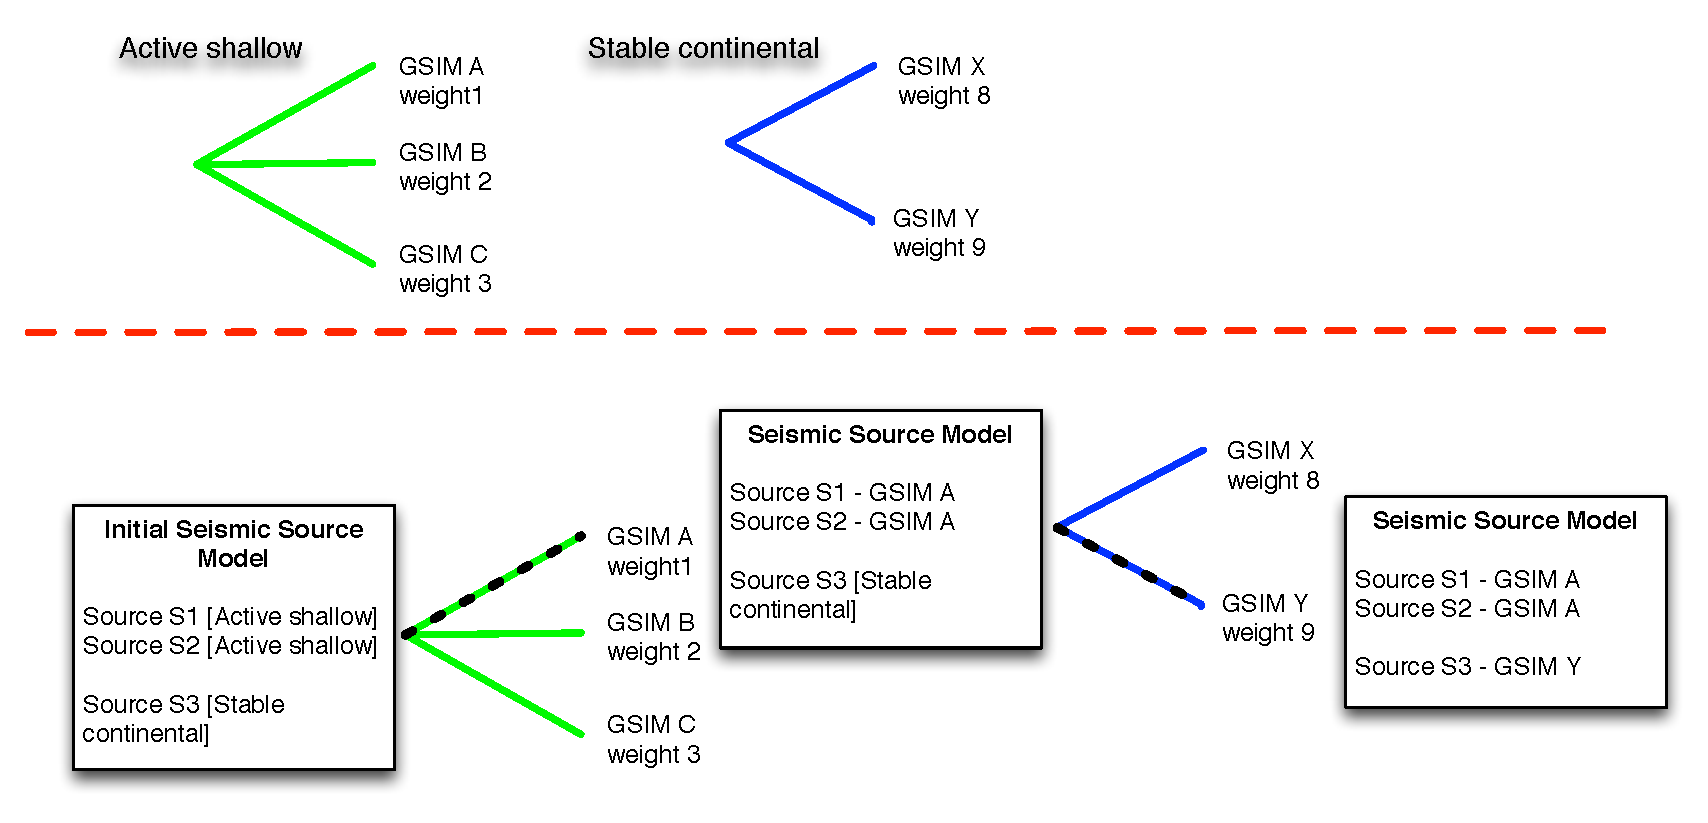
\includegraphics[width=\textwidth]{./Pictures/lts/logic_tree_gsim.pdf}
\caption{(upper panel) Example of branch sets belonging to the ground-motion 
logic tree. (lower panel) Example of ground-motion logic tree processing. 
The initial seismic source model, on the left,  is propagated through a simple 
logic tree structure following the path indicated by the black dashed line.
Model information is added incrementally as the input models propagate 
through the tree structure.}
\label{fig:logic_tree_gsim}
\end{figure}
% --------------------------------------------------------------------<<< Figure
%
%
% . . . . . . . . . . . . . . . . . . . . . . . . . . . . . . . . . . . . . . .
\subsection{The ground-motion model logic tree}
The current structure of the ground-motion model logic tree is 
simple and designed to support just the use of alternative 
\glspl{acr:gsim} models for a single tectonic region.
%
\subsubsection{Supported epistemic uncertainties}
The epistemic uncertainty allowed for the \gls{acr:gsim} 
logic-tree are the following:
\begin{itemize}
    \item \emph{Ground shaking intensity models} \hfill \\
        This module assigns to each tectonic region one or many 
        \glspl{acr:gsim}. This branch set implicitly contains a 
        filter since it is applied only to the seismic sources 
        belonging to the corresponding tectonic region. The  
        example within Figure \ref{fig:logic_tree_gsim}) illustrate
        the common processing of the ground-motion logic tree operated
        by the\gls{acr:oqe}. In this example the source model 
        contains seismic sources included in two tectonic domains:
        active tectonics and stable continental. The branch set defined 
        for 'active shallow' is then applied just to sources 'S1 and 'S3' 
        while the branch set for sources in stable continental regions
        is utilised only for source 'S3'.
\end{itemize}
% ..............................................................................
\section{Logic tree processing}
% https://github.com/gem/oq-commonlib/blob/master/openquake/commonlib/logictree.py
The \gls{acr:oqe} currently provides two distinct ways to process 
logic-trees: full-path enumeration and Monte Carlo sampling. 

Full path enumeration is a methodology which generates all the 
models admitted by a logic tree structure. 
%
For this reason, the use of this methodology is feasible only when 
the logic tree structure is relatively simple, that is when the number 
of end branches is at maximum in the order of a few tens.

Monte Carlo sampling is instead a methodology which makes an extensive 
use of random number generation in order to selects a subset of models 
capable to reliably define the overall uncertainty on the final results 
produced by the epistemic uncertainties used in the construction of the 
logic tree structure. 

In the following sections we provide a short description of 
the these two methodologies as implemented in the \gls{acr:oqe}.
%
% -------------------------------------------------------------------->>> Figure
\begin{figure}[ht]
\centering
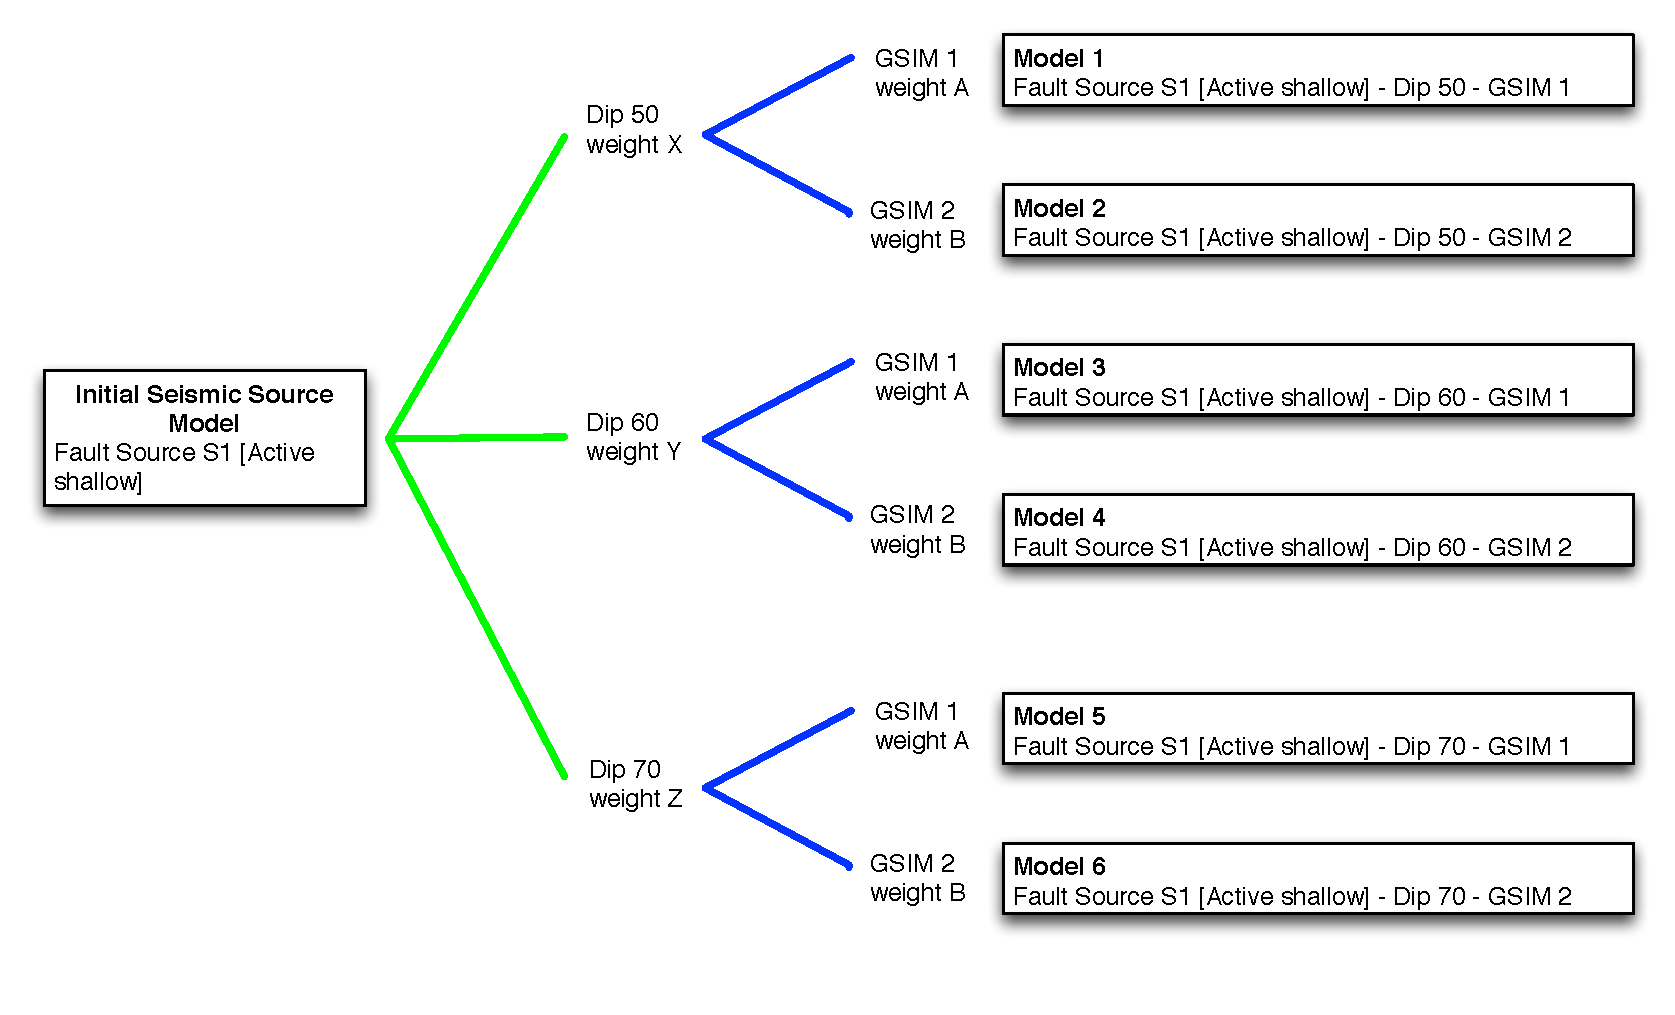
\includegraphics[width=\textwidth]{./Pictures/lts/logic_tree_ex1.pdf}
\caption{Logic tree full path enumeration processing. Note that the
first branching level, the one dealing with the definition of the initial 
seismic source model is neglected since we assume there is no epistemic
uncertainty associated with its definition. The final PSHA input model 
contains the initial sources each one with an associated GSIM to be used 
in the calculation of hazard for this specific logic tree path.}
\label{fig:logic_tree_example1}
\end{figure}
% --------------------------------------------------------------------<<< Figure
%
% . . . . . . . . . . . . . . . . . . . . . . . . . . . . . . . . . . . . . . .
\subsection{Full-path enumeration}
Full-path enumeration is the simplest methodology implemented in the
\gls{acr:oqe} for logic-tree processing. 
%
As previously anticipated, it consists on computing hazard 
for the entire set of investigated sites using all the possible paths 
admitted by the specific logic tree structure defined.

Let's consider the example described in Figure \ref{fig:logic_tree_example1}.
to illustrate how this method operates.
%
The logic structure depicted in this Figure contains two branching 
levels each one including a single branch set. 
%
Note that for the sake of simplicity and clarity we assume that the first 
branching level (i.e. the one used to define the initial seismic source 
model) is not affected by epistemic uncertainty. 
%
Note also that the initial seismic source model contains only one fault 
source.
%
The branch set in the first branching level describes the epistemic 
uncertainty on the dip angle; three values, each one with an associated 
probability, are considered plausible. 
%
The second branch set describes the epistemic uncertainties associated with 
the modelling of ground-motion; two \glspl{acr:gsim} are admitted in this
case. 
%
On the right side of the figure the entire set of models originated by the 
logic tree structure are briefly described in terms of their 
distinctive parameters.
% . . . . . . . . . . . . . . . . . . . . . . . . . . . . . . . . . . . . . . .
\subsection{Monte Carlo sampling}
The Monte Carlo sampling of the logic tree is implemented in a simple and 
straightforward way. 

Given a branch set, following the same order used to add the branches 
we create a cumulative distribution function like the one represented 
by the blue bars in Figure \ref{fig:logic_tree_mc_samp}. 
%
A sample model is then obtained from this distribution simply via the 
generation of a random number (i.e. a real number in the interval 
[0.0, 1.0[) and the identification of the interval in the cumulative 
distribution which includes it. In Figure \ref{fig:logic_tree_mc_samp}
the endpoints of the intervals are represented with horizontal dashed
segments. Let's assume for example that the random number generator
gives a value equal to 0.6. As clearly visible on the y-axis,
this value falls within the interval relative to branch 'b9'. 
%
Following samples will be generated by repeating the same procedure as
many times as needed. Clearly the higher is the weight associate with 
a branch the higher will be its probability of being sampled. In the 
example figure the branch with the higher weight is 'b5'.

A full path over the logic tree structure is built starting from the 
initial seismic source model and repeating this sampling procedure 
at each branching level.
%
% -------------------------------------------------------------------->>> Figure
\begin{figure}[ht]
\centering
% left, bottom, right, top
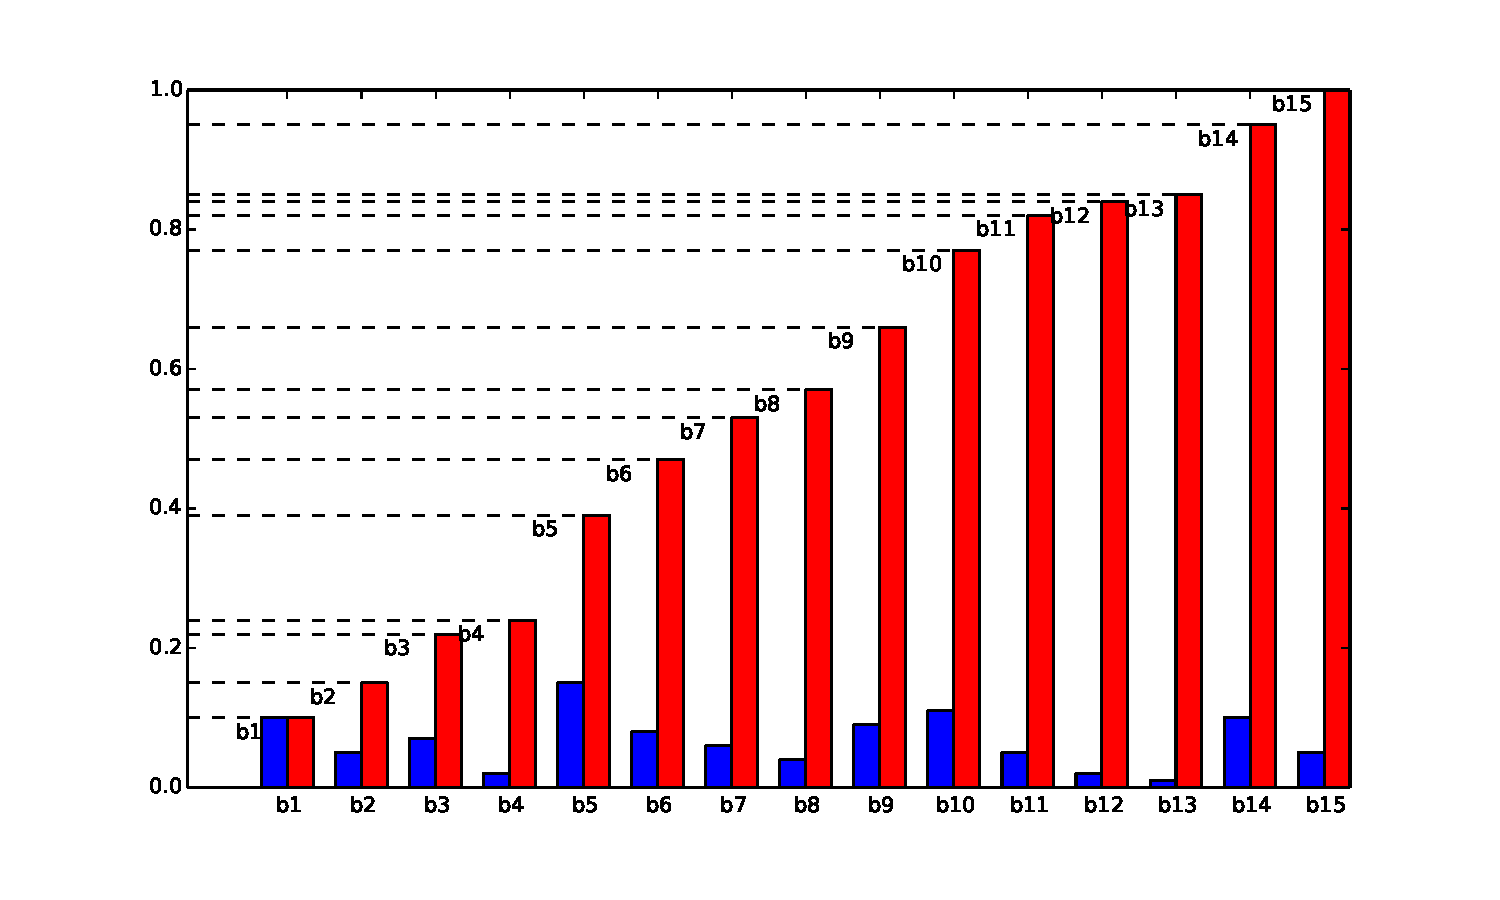
\includegraphics[trim = 20mm 5mm 5mm 10mm, clip, width=14cm]
    {./Pictures/lts/histogram_mc_sampl.pdf}
\caption{On the x-axis an hypothetical list of branches 
    included in a branch set. The height of the blue bar is proportional to 
    the corresponding weigth. The red bars show the cumulative distribution 
    function.}
\label{fig:logic_tree_mc_samp}
\end{figure}
% --------------------------------------------------------------------<<< Figure
%
% . . . . . . . . . . . . . . . . . . . . . . . . . . . . . . . . . . . . . . .
\subsection{Calculation of mean and percentiles/quantiles}
The calculation of statistical parameters for the computed result follows 
two distinct methodologies based on the logic tree processing methodology 
selected.
%
\clearpage
% ..............................................................................
\section{Future developments}
%
% . . . . . . . . . . . . . . . . . . . . . . . . . . . . . . . . . . . . . . .
\subsection{Logic tree pruning/collapsing}
